\begin{wrapfigure}[1]{r}[0cm]{4cm}
 \vspace{-6cm}
  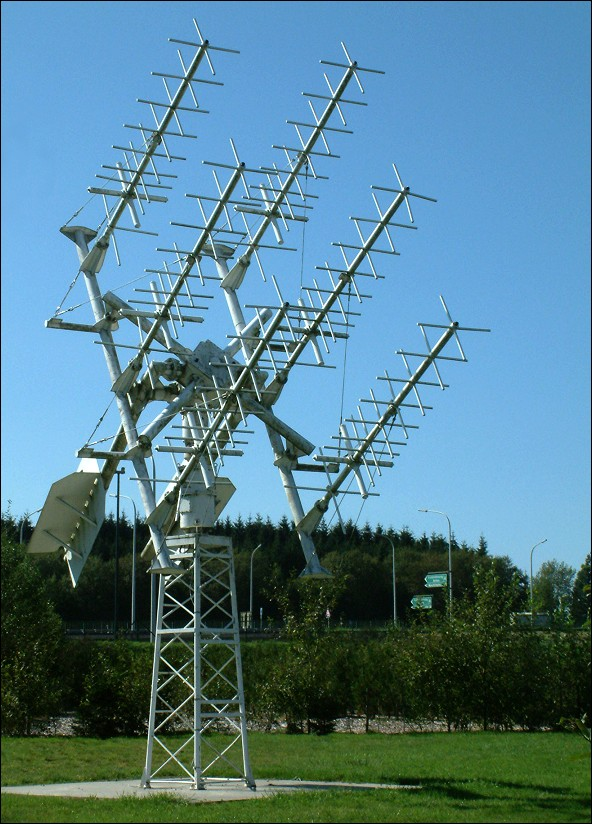
\includegraphics[scale=0.2]{Antennen/Bilder/Kreuzdipolarp.jpg}
 \vspace{-6cm}
\end{wrapfigure}

\section*{Theorie- und Prüfungsfragen}

\subsection*{Dipol}

\begin{enumerate} 
	\item \emph{\textbf{TH206}}  Ein Halbwellendipol wird auf der Grundfrequenz in der Mitte...
	\begin{enumerate}
	\itemsep1pt\parskip0pt\parsep0pt
		\item[A] spannungsgespeist.
		\item[B] stromgespeist.
		\item[C] endgespeist.
		\item[D] parallel gespeist.
		\loesung{Lösung B}
	\end{enumerate} 
	\item \emph{\textbf{TH204}}  Die Impedanz in der Mitte eines Halbwellendipols beträgt je nach Aufbauhöhe ungefähr ...
	\begin{enumerate}
	\itemsep1pt\parskip0pt\parsep0pt
		\item[A] 60 bis 120 Ohm.
		\item[B] 120 bis 240 Ohm.
		\item[C]  40 bis 80 Ohm.
		\item[D]  240 bis 600 Ohm.
		\loesung{Lösung C}
	\end{enumerate}
\end{enumerate}

\subsection*{EIRP und ERP}

\begin{enumerate} 
	\item[3] Was bedeutet der Ausdruck ERP.
		\loesung{ERP kommt von effective radio power und bedeutet ``Effektive Strahlungsleistung''}
	\item[4] Wie lässt sich die $P_{ERP}$ und $P_{EIRP}$ berechnen?
		\loesung{$P_{ERP} = (P_{Sender}-P_{Verlust}) \cdot G_{Antenne}; P_{EIRP}=1,64\cdot P_{ERP} $}
	\item[5] \emph{\textbf{TL204}}  Ein Sender mit 0,6 Watt Ausgangsleistung ist über eine Antennenleitung, die 1 dB Kabelverluste hat, an eine Richtantenne mit 11 dB Gewinn (auf Dipol bezogen) angeschlossen. Welche EIRP wird von der Antenne maximal abgestrahlt?
	\begin{enumerate}
	\itemsep1pt\parskip0pt\parsep0pt
		\item[A] $6,0W$
		\item[B] $7,8W$
		\item[C] $9,8W$
		\item[D] $12,7W$
		\loesung{Lösung C}
	\end{enumerate}
	\item[6] \emph{\textbf{TL205}}  Ein Sender mit 5 Watt Ausgangsleistung ist über eine Antennenleitung, die 2 dB Kabelverluste hat, an eine Antenne mit 5 dB Gewinn (auf Dipol bezogen) angeschlossen. Welche EIRP wird von der Antenne maximal abgestrahlt?
	\begin{enumerate}
	\itemsep1pt\parskip0pt\parsep0pt
		\item[A] $6,1W$
		\item[B] $10,0W$
		\item[C] $16,4W$
		\item[D] $32,8W$
		\loesung{Lösung C}
	\end{enumerate}
\end{enumerate}


\subsection*{Bauformen}

\begin{enumerate} 
\itemsep1pt\parskip0pt\parsep0pt
\item[7] Ordne der Abbildungen mit Schleifenantennen \ref{schleifen} folgende Bauformen zu: Dreiecksschleife (Delta Loop), Faltdipol, Quadratische Schleife (Quad Loop)
\loesung{
    Bild A zeigt einen Faltdipol.
    Bild B zeigt eine  Quadratische Schleife (Quad Loop).
    Bild C zeigt eine Dreiecksschleife (Delta Loop).
}
\end{enumerate}

\begin{figure}[H]
	\centering
	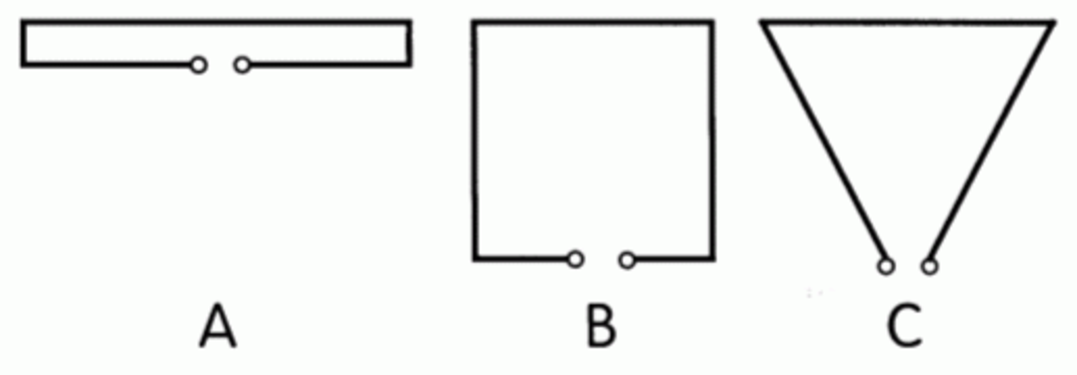
\includegraphics[scale=0.4]{Antennen/Bilder/Schleifen.pdf}
	\caption{Bauformen von Schleifenantennen}
	\label{schleifen}
\end{figure}

%------------------------------------------------------

\begin{enumerate} 
\itemsep1pt\parskip0pt\parsep0pt
\item[8] Ordne der Abbildungen mit UKW-Vertikalantennen \ref{ukw} folgende Bauformen zu: Groundplane-Antenne, Sperrtopf-Antenne, Viertelwellenstab, $\lambda/2$-Antenne, $5/8- \lambda$-Antenne
\loesung{
    Bild A zeigt einen Viertelwellenstab.
    Bild B zeigt eine  $\lambda/2$-Antenne.
    Bild C zeigt eine $5/8- \lambda$-Antenne.
    Bild D zeigt eine Sperrtopf-Antenne.
    Bild E zeigt eine Groundplane-Antenne.
}
\end{enumerate}

\begin{figure}[H]
	\centering
	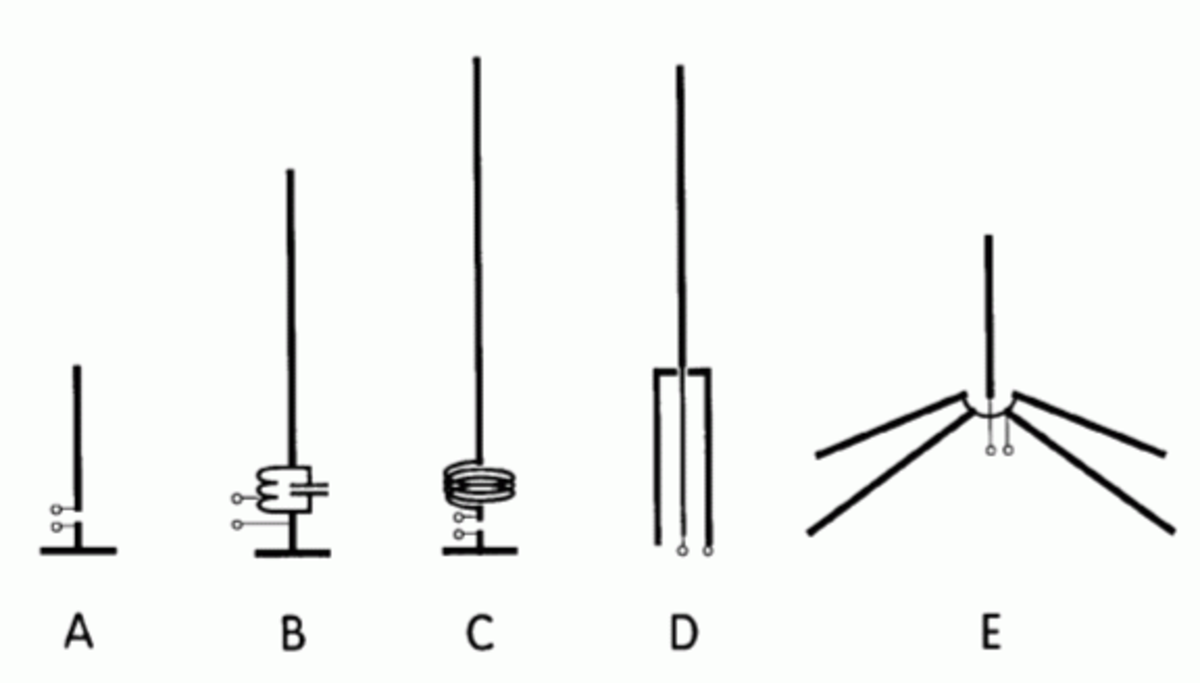
\includegraphics[scale=0.4]{Antennen/Bilder/ukw.pdf}
	\caption{Bauformen von UKW-Vertikalantennen}
	\label{ukw}
\end{figure}

%------------------------------------------------------

\begin{enumerate} 
\itemsep1pt\parskip0pt\parsep0pt
\item[9] Ordne der Abbildungen \ref{yagi} folgende Bauformen zu: horizontal polarisierte Yagi-Antenne, zirkular polarisierte X-Yagi-Antenne, Kreuz-Yagi-Antenne, vertikal polarisierte Yagi-Antenne.
\loesung{
    Bild A zeigt eine horizontal polarisierte Yagi-Antenne.
    Bild B zeigt eine vertikal polarisierte Yagi-Antenne.
    Bild C zeigt eine Kreuz-Yagi-Antenne.
    Bild D zeigt eine zirkular polarisierte X-Yagi-Antenne.
}
\end{enumerate}

\begin{figure}[H]
	\centering
	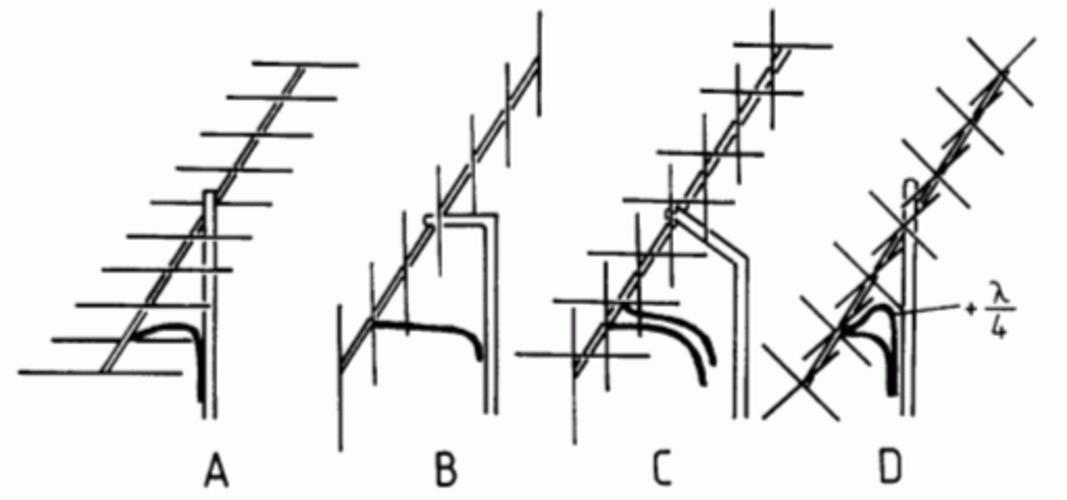
\includegraphics[scale=0.5]{Antennen/Bilder/TH209.pdf}
	\caption{Bauformen von Yagi-Antennen}
	\label{yagi}
\end{figure}
%------------------------------------------------------
\begin{enumerate} 
\itemsep1pt\parskip0pt\parsep0pt
\item[10] Ordne den Abbildungen \ref{strahlungsdiagramm} folgende Strahlungsdiagramme zu: Groundplane, Yagi-Antenne, Dipol, gibt es nicht.
\loesung{
    Bild A Dipol
    Bild B Yagi-Antenne
    Bild C Groundplane
    Bild D gibt es nicht
}
\end{enumerate}

\begin{figure}[H]
	\centering
	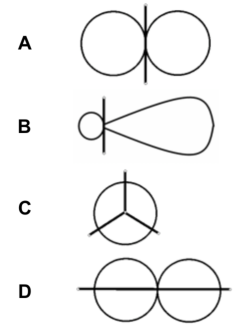
\includegraphics[scale=0.8]{Antennen/Bilder/Strahlungsdiagramm.pdf}
	\caption{Strahlungsdiagramme von Antennen}
	\label{strahlungsdiagramm}
\end{figure}
